\documentclass[11pt]{article}
\usepackage[margin=1in]{geometry}
\usepackage{amsmath,booktabs,graphicx,natbib,hyperref,xcolor,setspace}
\usepackage[T1]{fontenc}
\usepackage{lmodern}
\hypersetup{colorlinks=true,linkcolor=blue!50!black,citecolor=blue!50!black,urlcolor=blue!50!black}
\setstretch{1.15}
\bibliographystyle{apalike}

\title{Does the Weather Still Move Markets?\\[4pt]
\large A Pre-Registered, Two-Hemisphere, Post-Publication Test}
\author{Jason Li\thanks{E-mail: \href{mailto:lij62766@gmail.com}{lij62766@gmail.com}. The
pre-registrations, data pipeline and all code are available at \url{https://github.com/jasonstillchasin/does-weather-still-move-markets}. Each
pre-registration was committed to version control before the results it covers were estimated.}}
\date{Working paper --- \today}

\begin{document}
\maketitle

\begin{abstract}
\noindent
We re-examine weather and seasonal-mood effects in stock returns with two pre-registered studies,
free and replicable data, and a placebo-city inference procedure that directly addresses the
concern that weather effects are data-mined. Study~1 uses daily US (1955--2026) and Australian
(1984--2026) returns. After replicating \citet{hirshleifer2003} and \citet{kamstra2003} on their
own samples, one of nine primary tests survives multiple-testing correction and placebo inference:
New York cloud cover lowers same-day US returns by about 2 basis points per standard deviation
(Holm $p=0.029$); none of 100 placebo cities produces an effect as large. Study~2, pre-registered after
Study~1, pools 26 further exchanges and seven weather variables. Rain days lower returns (1.6 basis
points; Holm $p=0.045$, beyond all placebo draws), and high air pressure and sunshine point the same
way. However, the international cloud effect is absent after the \citet{hirshleifer2003} sample
ends, and every fair-weather effect is concentrated before 2003. Seasonal affective disorder
effects do not appear in the southern hemisphere, and temperature does not move markets. Weather
effects were small, and evidence that they persisted after publication is weak; a simple
cloud-timed trading strategy is not profitable after plausible transaction costs.
\end{abstract}

\noindent\textbf{Keywords:} weather, investor mood, seasonal affective disorder, pre-registration,
replication, placebo inference\\
\textbf{JEL:} G12, G14, G41

\newpage
\section{Introduction}

Few findings in behavioural finance are as memorable, or as contested, as the claim that sunshine
lifts stock prices. \citet{saunders1993} reported that New York Stock Exchange returns were lower
on cloudy days in New York; \citet{hirshleifer2003} extended the result to 26 exchanges;
\citet{kamstra2003} argued that seasonal affective disorder (SAD) produces a seasonal cycle in
returns that reverses between hemispheres; and \citet{cao2005} linked low temperatures to higher
returns. Each finding was challenged soon after publication. \citet{trombley1997} showed that the
New York effect was sensitive to the sample and the definition of cloudiness;
\citet{jacobsen2008} argued that SAD and temperature effects are hard to distinguish from the
Halloween effect of \citet{bouman2002}; \citet{kelly2010} questioned the construction of the SAD
variable; and \citet{novymarx2014} showed that a researcher free to choose predictors can find
``significant'' relations with sunspots and planetary alignments. For Australia, the evidence has
always been weak \citep{keef2007,worthington2009}.

Two decades later the question can be asked in a way that was not possible when these papers were
written. More than twenty years of data have accumulated since publication, which gives a genuine
out-of-sample test in the spirit of \citet{mclean2016}. Pre-registration makes it possible to
commit to specifications before seeing the new data. And free, long, hourly weather records for
any city on Earth make it possible to ask how unusual the New York result is relative to the
weather in cities that have nothing to do with the US market.

This paper makes four contributions. First, it pre-registers nine primary tests covering cloud
cover, temperature and SAD in the US and Australia, their post-publication persistence, a
market-structure channel and a small-stock channel, together with a decision rule that requires
both a multiple-testing-adjusted $p$-value and a placebo percentile. Second, it introduces a
placebo-city test: the same regression is estimated with weather from 100 cities outside the US
and Australia, and the real city's coefficient is ranked within that distribution. Because the
placebo cities share the seasonal structure of weather but not any plausible link to the market,
the test speaks directly to the data-mining critique. Third, it uses the reversal of seasons
between hemispheres to separate a seasonal-mood channel from calendar effects. Fourth, a second
study, pre-registered after the first study's results were known and run on 26 exchanges whose
returns had not been examined, tests seven weather variables (cloud, sunshine, temperature, wind,
rain, humidity and pressure) and gives an out-of-sample test of the international results of
\citet{hirshleifer2003}.

The results are mixed in an informative way. The New York cloud effect survives: $-2.1$ basis
points (bp) per standard deviation of cloud cover over 1955--2026, significant after Holm and
Romano--Wolf corrections, and more extreme than every one of 100 placebo cities. But the effect is
small, imprecisely estimated after 2003, not visible in Australian data after 2003, and a simple
strategy based on it loses money after costs. SAD does not appear in Australia, and temperature does not move the
market, although warm days lower the returns of energy and utility stocks, consistent with a
physical demand channel rather than mood. Across 26 further exchanges, rain days lower returns and
high pressure and sunshine raise them, with rain surviving the full decision rule; but the
evidence for these effects comes mainly from before 2003, and the international cloud effect is not
detectable after 1997.

\section{Hypotheses}

Table~\ref{tab:primary} lists the nine primary tests; the full pre-registration, including the
power analysis and decision rule, is in the online repository. All tests are one-sided in the
direction the original literature predicts.

\begin{description}
\item[H1] Deseasonalised cloud cover in the exchange city lowers same-day index returns (New York
for the US, Sydney for Australia).
\item[H2] The cloud effect survives publication: its coefficient after July 2003 is negative.
\item[H3] In Australia, the SAD effect follows the local (southern-hemisphere) season rather than
the New York calendar.
\item[H4] A temperature anomaly lowers returns \citep{cao2005}.
\item[H5] The New York weather effect weakens after the NYSE Hybrid Market (January 2007) moved
most trading off the floor.
\item[H6] Cloud effects are stronger in small stocks, whose investors are more local and more
retail \citep{loughran2004}.
\end{description}

\noindent A primary hypothesis is \emph{supported} only if its one-sided HAC $p$-value survives a
Holm correction at family-wise $\alpha=0.05$ and the placebo-city percentile lies in the predicted
5\% tail; \emph{inconclusive} if only one holds; and \emph{not supported} otherwise. With daily
return volatility near 1\% and about 5,800 post-2003 days, the minimum detectable effect at 80\%
power is roughly 3.3 bp per standard deviation, about the size of the original estimates. A
post-publication null is therefore informative only through its confidence interval, which we
report throughout.

\section{Data}

\paragraph{Returns.} US returns are the daily Center for Research in Security Prices (CRSP)
value-weighted market return (market excess return plus the risk-free rate) from Kenneth French's
data library \citep{french_data}; size and industry portfolios come from the same source.
Australian returns are the S\&P/ASX All Ordinaries price index from 1984 \citep{yahoo}. No free
daily total-return series covers 1984--2019, and the Reserve Bank of Australia table named in our
pre-registration no longer reports dividend yields, so the primary series adds back dividends as
the average daily dividend return in each calendar month, estimated from the S\&P/ASX 200
total-return and price indices over 2019--2026 (deviation D3, fixed before results were seen).

This approximation cannot matter for the weather tests, for a simple reason. The add-back is a
deterministic function of the calendar month, so it can bias a weather coefficient only through
a correlation between the weather anomaly and the calendar month. Our anomalies are deseasonalised
by week of year, which makes that correlation close to zero by construction: $-0.006$ for cloud and
$-0.011$ for temperature. Appendix Table~\ref{tab:checks} confirms this directly. Every Australian
weather coefficient is unchanged, to within 0.1 bp, with price-only returns or with calendar-month
fixed effects, which absorb any month-specific add-back exactly. The one test that is seasonal by
design, SAD (H3), does depend on the add-back: $-1.4$ bp with dividends and $-0.4$ bp without.
Neither version is significant, and both have the wrong sign, so the conclusion is the same. All
returns are log returns in percent, and the sample ends on 31 August 2026.

\paragraph{Weather.} Hourly observations come from NOAA's Global Historical Climatology Network
hourly data set \citep{ghcnh} for New York LaGuardia (with JFK filling gaps), and from NOAA's
Integrated Surface Database \citep{smith2011} and the Iowa Environmental Mesonet METAR archive
\citep{iem} for Sydney Airport. Cloud cover is total
sky cover in oktas, and temperature is air temperature; both are averaged over 06:00--16:00 local
time, following \citet{hirshleifer2003}. Each variable is deseasonalised against a trailing
30-year climatology for the same ISO week, using only earlier years, and standardised. The
resulting anomalies are available from 1955 in New York and 1984 in Sydney. For placebo cities,
alternative cities and a single-source robustness check we use the ERA5 reanalysis
\citep{hersbach2020}, point time series from the Copernicus Climate Data Store
\citep{c3s_timeseries}, processed identically. Exact definitions are in
Appendix~\ref{app:implementation}. ERA5 cloud cover
correlates 0.85 with the LaGuardia station series at the daily frequency.

\paragraph{Seasonal variables.} Night length is computed astronomically for each exchange city's
latitude. $\mathrm{SAD}_t$ equals night length minus 12 hours during the local autumn and winter,
and zero otherwise; $\mathrm{FALL}_t$ is a local-autumn dummy \citep{kamstra2003}.

\section{Method}

Each test is an OLS regression of the daily return on the weather or seasonal variable and a fixed
set of controls: day-of-week dummies, turn-of-year, pre- and post-holiday, and tax-year-end dummies
(December in the US, June in Australia), and two lags of the dependent variable. Australian
regressions also control for the most recent completed US return, because the New York session
closes before Sydney opens. Standard errors are Newey--West with five lags \citep{newey1987}.
Multiplicity across the nine tests is handled with the Holm procedure \citep{holm1979}, with a
Romano--Wolf stepdown \citep{romano2005} based on a joint stationary bootstrap \citep{politis1994}
as robustness. Bandwidths, bootstrap settings, random seeds, the handling of missing data and
holidays, and the exact standardisation formula are given in Appendix~\ref{app:implementation}.
Every table and figure can be regenerated from the raw downloads with a single command
(\texttt{make all}).

The placebo-city test re-estimates each weather regression 100 times, each time using ERA5 cloud or
temperature anomalies for a different city more than 1,000 km from both New York and Sydney (the
list was fixed in the pre-registration). The real city is re-estimated with ERA5 data as well, so
the comparison is like for like. We report the number of placebo coefficients at least as extreme.
With 100 placebo cities, the resolution of this test is one percentage point, so ``0/100'' means an
empirical placebo percentile below 1\%, not a probability of zero. A second placebo shifts the real station's weather series by $k=1,\dots,30$ years. This
preserves seasonality exactly and breaks only the day-to-day link.

\section{Results}

\subsection{Replication}

Table~\ref{tab:replication} shows that our data reproduce the original findings on the original
samples. In a logit of up days on deseasonalised New York cloud cover over 1982--1997, the
coefficient is $-0.114$ ($t=-3.56$), matching the sign and significance of
\citet{hirshleifer2003}. Over 1928--2000, the SAD coefficient is positive (2.2 bp per hour of
night beyond 12, $t=2.77$) and the autumn dummy negative ($-5.0$ bp, $t=-2.31$), as in
\citet{kamstra2003}. Any failure of the extended tests therefore cannot be blamed on data that
cannot reproduce the originals.

\begin{table}[htbp]\centering\footnotesize
\caption{Replication gate (data up to 2000). Pass = predicted sign with one-sided $p<0.10$.}
\label{tab:replication}
\begin{tabular}{lcrrrr}\toprule
Specification & Pred. & $\beta$ (bp) & $t$ & $p$ & $N$ \\ \midrule
HS 2003 NYC logit (1982-97) & $<$0 & -11.41 & -3.56 & $<$0.001 & 4,012 \\
HS 2003 NYC OLS (1982-97) & $<$0 & -2.01 & -1.26 & 0.105 & 4,012 \\
KKL 2003 US SAD (1928-2000) & $>$0 & +2.15 & +2.77 & 0.003 & 19,411 \\
KKL 2003 US FALL (1928-2000) & $<$0 & -5.01 & -2.31 & 0.011 & 19,411 \\
KKL 2003 US SAD + weather (1955-2000) & $>$0 & +2.63 & +3.00 & 0.001 & 9,389 \\
KKL 2003 US FALL + weather (1955-2000) & $<$0 & -3.34 & -1.46 & 0.072 & 9,389 \\
\bottomrule\end{tabular}\end{table}


\subsection{Primary tests}

Table~\ref{tab:primary} reports the nine pre-registered tests. Only H1 in the US is supported. A
one-standard-deviation increase in New York cloud cover lowers the same-day market return by 2.1
bp (95\% CI $[-3.7,-0.6]$). The Holm-adjusted $p$-value is 0.029 and the Romano--Wolf $p$-value
0.035. Figure~\ref{fig:placebo} shows the placebo distribution: centred almost exactly on zero
(mean $-0.03$ bp, standard deviation 0.66 bp), with the New York ERA5 coefficient ($-1.9$ bp)
beyond every placebo city. None of the 30 year-shifted series produces a coefficient as negative
either.

In Australia the Sydney cloud coefficient has the same sign and similar size ($-1.8$ bp), and only
2 of 100 placebo cities are as extreme, but it does not survive the Holm correction, so H1-AU
is inconclusive.

\begin{table}[htbp]\centering\footnotesize
\caption{Pre-registered primary tests. $\beta$ in basis points per one-standard-deviation weather shock (for H3, per hour of night beyond 12). One-sided HAC $p$-values in the predicted direction; Holm and Romano--Wolf adjust across the nine tests. Placebo = number of the 100 placebo cities with a coefficient at least as extreme (ERA5); Shift = number of the 30 year-shifted weather series at least as extreme.}
\label{tab:primary}
\resizebox{\textwidth}{!}{%
\begin{tabular}{llrcrrrrrrl}\toprule
ID & Hypothesis & $\beta$ & 95\% CI & $t$ & $p_1$ & Holm & R--W & Placebo & Shift & Verdict \\ \midrule
H1-US & NYC cloud lowers US returns & -2.13 & [-3.7, -0.6] & -2.72 & 0.003 & 0.029 & 0.035 & 0/100 & 0/30 & Supported \\
H1-AU & Sydney cloud lowers AU returns & -1.77 & [-3.6, +0.1] & -1.87 & 0.031 & 0.246 & 0.224 & 2/100 & 1/30 & Inconclusive \\
H2-US & US cloud effect after 2003 & -1.95 & [-5.2, +1.3] & -1.18 & 0.119 & 0.834 & 0.619 & 17/100 & 5/30 & Not Supported \\
H2-AU & AU cloud effect after 2003 & +0.07 & [-2.3, +2.4] & +0.06 & 0.523 & 1.000 & 0.982 & 50/100 & 16/30 & Not Supported \\
H3-AU & AU SAD follows the season & -1.38 & [-3.9, +1.2] & -1.06 & 0.855 & 1.000 & 0.982 & -- & -- & Not Supported \\
H4-US & NYC temperature lowers returns & +0.13 & [-1.2, +1.5] & +0.19 & 0.574 & 1.000 & 0.982 & 50/100 & 18/30 & Not Supported \\
H4-AU & Sydney temperature lowers returns & +0.67 & [-0.9, +2.2] & +0.85 & 0.803 & 1.000 & 0.982 & 87/100 & 28/30 & Not Supported \\
H5-US & Effect weakens after NYSE Hybrid & +0.18 & [-3.9, +4.3] & +0.09 & 0.465 & 1.000 & 0.982 & 36/100 & 18/30 & Not Supported \\
H6-US & Stronger in small minus big & -0.07 & [-1.2, +1.1] & -0.11 & 0.454 & 1.000 & 0.982 & 10/100 & 12/30 & Not Supported \\
\bottomrule\end{tabular}}\end{table}


\begin{figure}[htbp]\centering
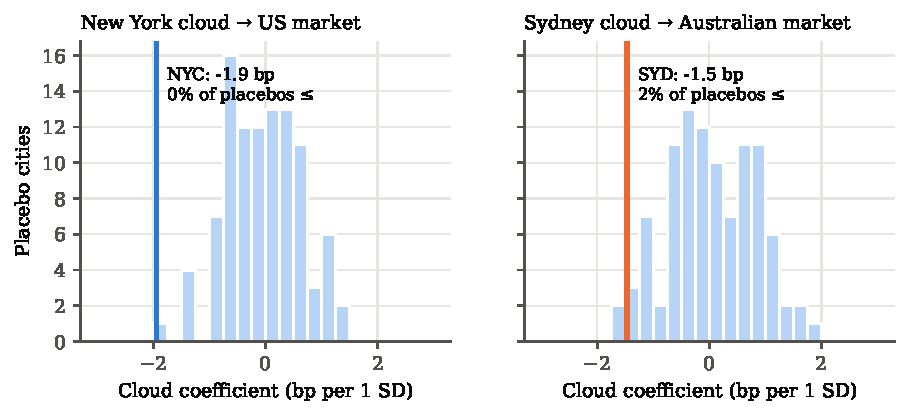
\includegraphics[width=\textwidth]{figs/placebo_h1.pdf}
\caption{Placebo-city distributions for the cloud coefficient (H1). Bars show coefficients
estimated with ERA5 cloud anomalies from 100 placebo cities; the vertical line is the exchange
city, also measured with ERA5.}
\label{fig:placebo}
\end{figure}

\paragraph{After publication.} The post-2003 US coefficient is $-2.0$ bp, almost identical to the
full-sample estimate, but its confidence interval ($[-5.2,+1.3]$) cannot distinguish persistence
from disappearance. For Australia the post-2003 coefficient is $+0.1$ bp with a much tighter
interval ($[-2.3,+2.4]$). Figure~\ref{fig:rolling} shows trailing ten-year estimates. The New York
coefficient is negative in most windows but close to zero for windows ending 2005--2012. The
Sydney coefficient drifts from about $-3$ bp in the 1990s towards zero after 2015.

\begin{figure}[htbp]\centering
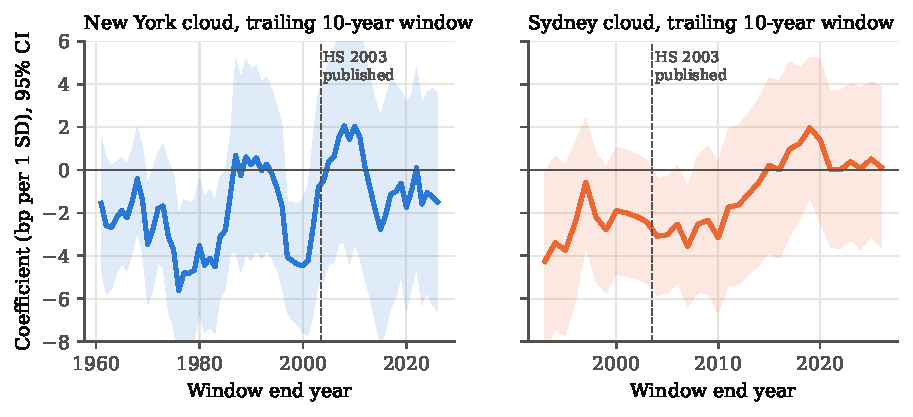
\includegraphics[width=\textwidth]{figs/rolling_cloud.pdf}
\caption{Trailing ten-year estimates of the cloud coefficient, with 95\% HAC confidence bands. The
dashed line marks the publication of \citet{hirshleifer2003}.}
\label{fig:rolling}
\end{figure}

\paragraph{Seasons, temperature and channels.} The Australian SAD coefficient has the wrong sign
($-1.4$ bp per hour, $t=-1.06$), so the seasonal-mood cycle does not follow the southern-hemisphere
season (H3). Temperature anomalies have no detectable effect in either market (H4). There is no
evidence that the New York effect weakened when floor trading declined (H5), although the
interaction is imprecise, nor that it is concentrated in small stocks (H6).

\subsection{Robustness and exploratory results}

Table~\ref{tab:robust_weather} (appendix) varies the US and Australian cloud and temperature
specifications. The US cloud result holds with ERA5 weather ($-1.9$ bp), full-sample
deseasonalisation ($-2.1$ bp), a logit of up days ($t=-3.73$) and a GARCH(1,1) model with
Student-$t$ errors ($-2.1$ bp, $t=-4.24$). It is weaker with Chicago weather ($-1.2$ bp, $t=-1.61$),
as expected if the relevant weather is where the market is. In a split sample, the coefficient is
$-2.1$ bp ($t=-2.53$) over 1955--2006 and $-1.9$ bp ($t=-0.97$) over 2007--2026. Rain during
trading hours lowers US returns by 5.4 bp ($t=-2.86$), consistent with the cloud result.

The Australian cloud coefficient is robust to price-only returns and ERA5 data, but Melbourne weather
shows nothing ($+0.2$ bp). Every post-2003 Australian variant is within 0.6 bp of zero.

Table~\ref{tab:robust_seasonal} examines seasonal effects. In the US, the SAD coefficient is
positive over 1955--2026 (2.0 bp, $t=2.40$) and similar but insignificant after 2003. In
Australia, neither the local SAD variable (0.2 bp) nor the New York-calendar SAD variable
($-0.2$ bp) nor a Halloween dummy (1.4 bp, $t=0.86$) is significant, so the reversed-season test
favours neither the mood nor the calendar account. It simply finds no seasonal cycle.

Table~\ref{tab:robust_industry} provides suggestive evidence for a physical channel. Controlling
for the same-day market return, warmer-than-normal days lower the returns of the oil industry
($-2.0$ bp, $t=-2.87$) and of utilities ($-1.0$ bp, $t=-2.25$). This is consistent with lower
heating demand rather than investor mood. Cloudy days raise coal-industry returns (5.6 bp,
$t=3.82$). These are sixteen exploratory tests, so only the coal and oil results clear a
Bonferroni threshold.

\subsection{Economic significance}

Table~\ref{tab:strategy} asks whether the effect can be traded. Using the SPY exchange-traded fund
from 1993, we hold the market from open to close only on days whose early-morning (06:00--10:00)
New York cloud cover is below normal. The open-to-close return on sunny mornings exceeds that on
cloudy mornings by only 0.3 bp per day ($t=0.13$). With a 1 bp round-trip cost, every variant
loses money. This specified cloud-timed SPY strategy is therefore not profitable after plausible
round-trip transaction costs. We have not searched over other implementations (futures, other
markets, other weather signals), and we do not claim that no weather-based strategy could ever be
profitable. The result is consistent with the conclusion of \citet{hirshleifer2003} that the
effect is too small to trade.

\begin{table}[htbp]\centering\footnotesize
\caption{Cloud-timed SPY open-to-close strategy, 1993--2026. Long SPY from the open to the close on days whose 06:00--10:00 New York cloud anomaly is below zero (``sunny''), or above it (``cloudy''); otherwise in cash (zero return). Costs are per round trip.}
\label{tab:strategy}
\begin{tabular}{lrrrr}\toprule
Rule & Cost (bp) & Ann.\ return (\%) & Sharpe & Days held \\ \midrule
every day & 0 & +0.71 & +0.05 & 8,430 \\
sunny mornings only & 0 & +0.45 & +0.05 & 3,381 \\
cloudy mornings only & 0 & +0.25 & +0.02 & 5,049 \\
every day & 1 & -1.81 & -0.12 & 8,430 \\
sunny mornings only & 1 & -0.56 & -0.06 & 3,381 \\
cloudy mornings only & 1 & -1.25 & -0.11 & 5,049 \\
every day & 2 & -4.33 & -0.29 & 8,430 \\
sunny mornings only & 2 & -1.57 & -0.17 & 3,381 \\
cloudy mornings only & 2 & -2.76 & -0.23 & 5,049 \\
\midrule
\multicolumn{5}{l}{Sunny minus cloudy mornings: +0.28 bp per day ($t = 0.13$), $N = 8,430$} \\
\bottomrule\end{tabular}\end{table}


\section{Study 2: Seven weather variables across 26 exchanges}
\label{sec:study2}

\subsection{Design}

Study~2 was pre-registered (\texttt{prereg/study2\_preregistration.md}) after Study~1 was
complete, and frozen before any return from the new exchanges was examined. We began with a list
of 37 national benchmark indices and kept the 26 whose free daily history starts by 2006 and has
fewer than 5\% zero-change days: twelve in Europe, nine in Asia, four in the Americas and one in
New Zealand. Appendix~\ref{app:exchanges} gives the eligibility algorithm, the full candidate list
and the reason for each exclusion. New
York and Sydney are excluded from the primary tests because their results were already known. For
every city, seven weather variables come from ERA5 and are processed identically: mean cloud cover,
solar radiation (``sunshine''), temperature, wind speed, relative humidity and sea-level pressure,
each as a trailing-climatology $z$-score over 06:00--16:00 local time, plus a rain-day indicator
($\geq 1$~mm) measured relative to its climatological frequency. Returns are scaled by each index's
trailing 60-day volatility, so coefficients are in percent of a daily standard deviation, and
estimated in a pooled regression with exchange fixed effects and Driscoll--Kraay standard errors,
which allow for correlation across markets on the same day. The decision rule is the same as in
Study~1. The placebo test gives each exchange the weather of a random city more than 1,000 km
away, 200 times.

\subsection{Results}

Table~\ref{tab:s2primary} reports the nine primary tests. Rain is supported: a rain day lowers
returns by 1.6\% of a daily standard deviation (about 1.6 bp at the median volatility; Holm
$p=0.045$), and none of the 200 placebo assignments produces an effect as large (empirical
percentile below 0.5\%). High pressure (+1.0 bp per
standard deviation, Holm $p=0.070$), sunshine (+0.6 bp), cloud ($-0.4$ bp) and humidity ($-0.4$ bp)
all lie in the extreme tail of their placebo distributions but do not survive the Holm correction,
so they are inconclusive. Their signs are consistent: fair weather goes with higher returns.
Temperature, wind and SAD show nothing. The SAD test has little power, however, since only four
exchanges are in the southern hemisphere.

The out-of-sample cloud test (S2) is clearly negative. Using only data from 1998, after the
\citet{hirshleifer2003} sample ends, the pooled cloud coefficient is $-0.2$ bp ($t=-0.57$) and sits in
the middle of its placebo distribution.

\begin{table}[htbp]\centering\footnotesize
\caption{Study 2 pre-registered primary tests, pooled over 26 exchanges not used in Study 1. $\beta$ is in percent of a daily return standard deviation per one-SD weather shock (rain: per rain day relative to its climatological frequency); bp converts at the median daily volatility. Driscoll--Kraay standard errors. Placebo = number of the 200 random placebo-city assignments at least as extreme.}
\label{tab:s2primary}
\resizebox{\textwidth}{!}{%
\begin{tabular}{llrrrrrrrl}\toprule
ID & Weather variable & $\beta$ (\% SD) & bp & $t$ & $p$ & Holm & Placebo & $N$ & Verdict \\ \midrule
S1 & Cloud (full sample) & -0.39 & -0.41 & -1.49 & 0.068 & 0.410 & 1/200 & 222,941 & Inconclusive \\
S2 & Cloud, 1998 onward & -0.16 & -0.17 & -0.57 & 0.284 & 1.000 & 34/200 & 184,234 & Not Supported \\
S3 & Sunshine & +0.55 & +0.58 & +2.14 & 0.016 & 0.113 & 2/200 & 222,941 & Inconclusive \\
S4 & Temperature & -0.12 & -0.13 & -0.39 & 0.349 & 1.000 & 78/200 & 222,941 & Not Supported \\
S5 & Wind & -0.11 & -0.12 & -0.41 & 0.342 & 1.000 & 110/200 & 222,941 & Not Supported \\
S6 & Rain day & -1.55 & -1.64 & -2.58 & 0.005 & 0.045 & 0/200 & 222,941 & Supported \\
S7 & Humidity (two-sided) & -0.42 & -0.44 & -1.66 & 0.097 & 0.484 & 5/200 & 222,941 & Inconclusive \\
S8 & Pressure (two-sided) & +0.93 & +0.98 & +2.62 & 0.009 & 0.070 & 0/200 & 222,941 & Inconclusive \\
S9 & SAD follows local season & +0.13 & +0.14 & +0.22 & 0.412 & 1.000 & -- & 222,941 & Not Supported \\
\bottomrule\end{tabular}}\end{table}


Table~\ref{tab:s2splits} and Figure~\ref{fig:s2decay} show why. The evidence for every
fair-weather effect comes mainly from the period before July 2003. The rain coefficient falls from $-3.8\%$ of a standard
deviation ($t=-3.9$) to $-0.3\%$ ($t=-0.4$), sunshine from $+1.8\%$ ($t=4.2$) to $-0.1\%$, and cloud
from $-1.2\%$ ($t=-2.6$) to zero. Pressure declines least, from $+1.5\%$ to $+0.7\%$ ($t=1.5$). The
post-2003 intervals are wide enough that smaller persistent effects cannot be excluded; what the
data show is that the effects are not detectable after 2003, not that they are exactly zero. The
effects are found in developed rather than emerging markets and in the northern hemisphere. When all
seven variables enter one regression, only pressure remains significant ($t=2.1$). This suggests
that the fair-weather pattern reflects high-pressure weather systems more than any single
variable.

\begin{figure}[htbp]\centering
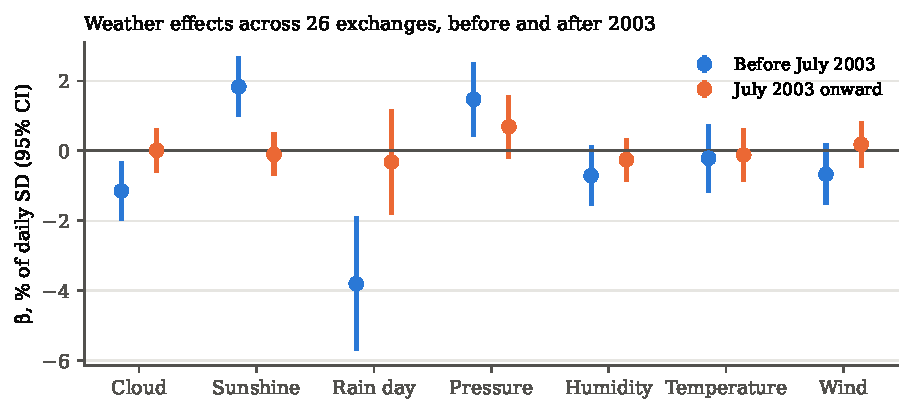
\includegraphics[width=\textwidth]{figs/s2_decay.pdf}
\caption{Pooled Study~2 coefficients before and after July 2003, with 95\% Driscoll--Kraay
confidence intervals.}
\label{fig:s2decay}
\end{figure}

\begin{table}[htbp]\centering\footnotesize
\caption{Study 2 exploratory splits (26 exchanges). Cells: $\beta$ in percent of a daily SD, with $t$-statistics in parentheses. ``Joint'' enters all seven anomalies in one regression.}
\label{tab:s2splits}
\resizebox{\textwidth}{!}{%
\begin{tabular}{lrrrrrrr}\toprule
Variable & Pre-2003 & Post-2003 & Developed & Emerging & Northern & Southern & Joint \\ \midrule
Cloud & -1.15 (-2.6) & +0.01 (+0.0) & -0.51 (-1.5) & -0.18 (-0.5) & -0.46 (-1.6) & -0.00 (-0.0) & +0.08 (+0.2) \\
Sunshine & +1.83 (+4.2) & -0.10 (-0.3) & +0.71 (+2.1) & +0.28 (+0.8) & +0.60 (+2.2) & +0.24 (+0.4) & +0.33 (+0.8) \\
Temperature & -0.21 (-0.4) & -0.12 (-0.3) & -0.21 (-0.5) & +0.05 (+0.1) & -0.07 (-0.2) & -0.32 (-0.5) & -0.09 (-0.2) \\
Wind & -0.67 (-1.5) & +0.18 (+0.5) & -0.31 (-0.8) & +0.22 (+0.6) & -0.11 (-0.4) & -0.10 (-0.2) & +0.13 (+0.5) \\
Rain day & -3.80 (-3.9) & -0.32 (-0.4) & -1.71 (-2.2) & -1.20 (-1.3) & -1.85 (-2.8) & +0.15 (+0.1) & -0.76 (-1.0) \\
Humidity & -0.71 (-1.6) & -0.26 (-0.8) & -0.53 (-1.5) & -0.24 (-0.7) & -0.46 (-1.6) & -0.26 (-0.4) & +0.02 (+0.0) \\
Pressure & +1.47 (+2.7) & +0.69 (+1.5) & +1.64 (+3.4) & -0.17 (-0.4) & +1.09 (+2.8) & +0.00 (+0.0) & +0.81 (+2.1) \\
\bottomrule\end{tabular}}\end{table}


Figure~\ref{fig:s2heatmap} shows the exchange-level estimates. Twelve of the 196 exchange--variable
tests survive a Benjamini--Hochberg false-discovery rate of 10\%. Pressure effects appear in
London, Frankfurt, Paris, Zurich and Brussels, but these cities share weather systems, so they are
closer to a single European finding than to five. Tokyo and Taipei show cloud and sunshine effects
like New York's. Among the other exploratory results, storm and heat days have no effect on
returns, and warmer-than-normal days are associated with lower volatility ($t=-2.8$).

\begin{figure}[htbp]\centering
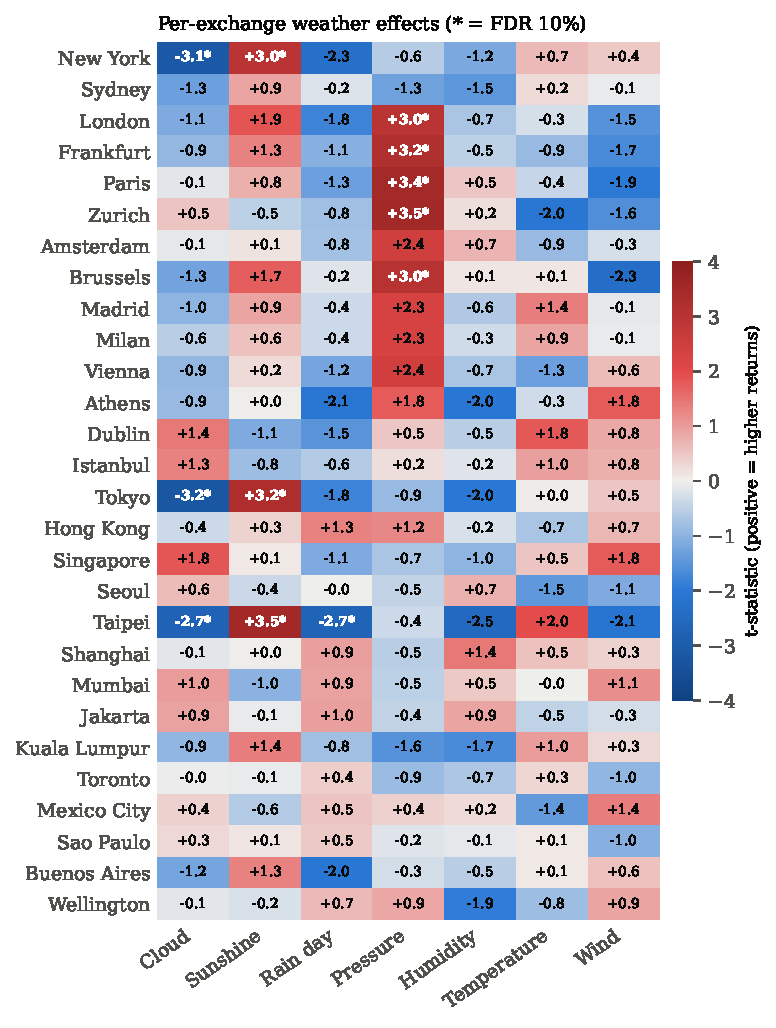
\includegraphics[width=0.72\textwidth]{figs/s2_heatmap.pdf}
\caption{Exchange-level $t$-statistics for each weather variable (volatility-scaled returns, HAC
standard errors). Positive values mean higher returns. Starred cells survive a
Benjamini--Hochberg false-discovery rate of 10\% across all 196 tests.}
\label{fig:s2heatmap}
\end{figure}

\section{Identification and limitations}
\label{sec:limits}

Weather is determined outside financial markets, so reverse causality is not a concern. But our
regressions identify an \emph{association} between local weather and returns, not the channel that
produces it. At least three channels are consistent with the results: investor mood, the one the
original literature proposed; physical effects on cash flows, which our industry results support
for temperature (oil and utilities); and weather-driven changes in local activity or attention,
such as fewer trades on rainy days. We do not separate these.

Several further limitations should be kept in mind. First, post-publication tests have limited
power: the post-2003 US cloud interval $[-5.2,+1.3]$ bp is consistent with both persistence and
disappearance. Second, ERA5 reanalysis and station records measure weather with error, which
biases coefficients towards zero. Third, Study~2 uses price indices, and the Australian total
return is approximated (Section~3). Fourth, the placebo tests have a resolution of 1/100 (Study~1)
and 1/200 (Study~2), and cities that share weather systems, such as those in Europe, provide less
independent evidence than their number suggests. Fifth, the Study~2 candidate list was compiled by
the author, although it was fixed before any of its returns were examined. Finally, both
pre-registrations were written and time-stamped by the author in version control. Their
credibility rests on the public commit history.

\section{Discussion and conclusion}

Pre-registration and placebo inference change how the old weather results should be read. In our
data, the New York cloud association is not an artefact of specification search. It replicates, survives
multiplicity adjustment, and is more extreme than the same statistic computed with the weather of
every one of 100 unrelated cities. But it is small, and most of the evidence for it comes from
before 2007. After publication the US estimate is similar in size but imprecise, and the
Australian estimate is close to zero, with a confidence interval tight enough to rule out effects
of the size originally reported. The SAD cycle does not appear in Australia, and temperature
matters only for industries whose cash flows depend on it. Study~2 generalises the picture. Across
26 further exchanges, fair weather (no rain, high pressure, sunshine) went with higher returns,
and rain survives the full pre-registered decision rule. But the evidence for these effects comes
mainly from before 2003, and the international cloud effect of \citet{hirshleifer2003} is not
detectable out of sample.

One possible interpretation is that the historical association reflected a localised mood channel,
which mattered when trading was concentrated among people who experienced the local weather and
has weakened as trading dispersed geographically and algorithmically. The decline in the Sydney
coefficient, the near-zero New York estimates in windows after 2005, and the concentration of the
Study~2 effects before 2003 fit this interpretation. However, our direct market-structure test (H5)
is too imprecise to confirm it, and the evidence is equally consistent with the other channels
discussed in Section~\ref{sec:limits}. Future work could use investor-location data
\citep{goetzmann2015} or intraday data around the electronic-trading transitions to sharpen the
test.

\bibliography{refs}

\clearpage
\appendix
\section{Additional tables}
\begin{table}[htbp]\centering\footnotesize
\caption{Robustness of the weather tests (exploratory; not multiplicity-adjusted).}
\label{tab:robust_weather}
\begin{tabular}{lcrrrr}\toprule
Specification & Pred. & $\beta$ (bp) & $t$ & $p$ & $N$ \\ \midrule
H1-US station (primary) & $<$0 & -2.13 & -2.72 & 0.003 & 17,736 \\
H1-US ERA5 weather & $<$0 & -1.94 & -2.56 & 0.005 & 18,036 \\
H1-US CHI weather (ERA5) & $<$0 & -1.24 & -1.61 & 0.054 & 18,036 \\
H1-US full-sample deseasonalisation & $<$0 & -2.07 & -2.90 & 0.002 & 19,028 \\
H1-US logit up/down & $<$0 & -5.79 & -3.73 & $<$0.001 & 17,736 \\
H1-US GARCH(1,1)-t mean & $<$0 & -2.10 & -4.24 & $<$0.001 & 17,736 \\
H1-AU station (primary) & $<$0 & -1.77 & -1.87 & 0.031 & 10,111 \\
H1-AU ERA5 weather & $<$0 & -1.47 & -1.68 & 0.046 & 10,633 \\
H1-AU MEL weather (ERA5) & $<$0 & +0.24 & +0.32 & 0.625 & 10,633 \\
H1-AU full-sample deseasonalisation & $<$0 & -2.03 & -2.10 & 0.018 & 10,111 \\
H1-AU AU price-only returns & $<$0 & -1.76 & -1.86 & 0.031 & 10,111 \\
H1-AU logit up/down & $<$0 & -4.11 & -1.76 & 0.039 & 10,111 \\
H1-AU GARCH(1,1)-t mean & $<$0 & -1.05 & -1.54 & 0.062 & 10,111 \\
H2-US station (primary) & $<$0 & -1.95 & -1.18 & 0.119 & 17,736 \\
H2-US ERA5 weather & $<$0 & -1.40 & -0.88 & 0.189 & 18,036 \\
H2-US CHI weather (ERA5) & $<$0 & -2.84 & -1.69 & 0.046 & 18,036 \\
H2-US full-sample deseasonalisation & $<$0 & -1.97 & -1.19 & 0.118 & 19,028 \\
H2-US break at 2001-01 (HS working paper) & $<$0 & -0.43 & -0.27 & 0.395 & 17,736 \\
H2-AU station (primary) & $<$0 & +0.07 & +0.06 & 0.523 & 10,111 \\
H2-AU ERA5 weather & $<$0 & -0.10 & -0.10 & 0.462 & 10,633 \\
H2-AU MEL weather (ERA5) & $<$0 & -0.06 & -0.06 & 0.477 & 10,633 \\
H2-AU full-sample deseasonalisation & $<$0 & -0.10 & -0.08 & 0.469 & 10,111 \\
H2-AU AU price-only returns & $<$0 & +0.06 & +0.05 & 0.521 & 10,111 \\
H2-AU break at 2001-01 (HS working paper) & $<$0 & -0.61 & -0.54 & 0.295 & 10,111 \\
H4-US station (primary) & $<$0 & +0.13 & +0.19 & 0.574 & 18,538 \\
H4-US ERA5 weather & $<$0 & +0.00 & +0.00 & 0.502 & 18,036 \\
H4-US CHI weather (ERA5) & $<$0 & +0.74 & +1.13 & 0.870 & 18,036 \\
H4-US full-sample deseasonalisation & $<$0 & -0.06 & -0.09 & 0.463 & 19,938 \\
H4-US logit up/down & $<$0 & +2.09 & +1.46 & 0.928 & 18,538 \\
H4-US GARCH(1,1)-t mean & $<$0 & +0.56 & +1.28 & 0.899 & 18,538 \\
H4-AU station (primary) & $<$0 & +0.67 & +0.85 & 0.803 & 10,610 \\
H4-AU ERA5 weather & $<$0 & +0.80 & +0.98 & 0.837 & 10,633 \\
H4-AU MEL weather (ERA5) & $<$0 & +0.78 & +1.02 & 0.847 & 10,633 \\
H4-AU full-sample deseasonalisation & $<$0 & +0.49 & +0.60 & 0.725 & 10,610 \\
H4-AU AU price-only returns & $<$0 & +0.68 & +0.87 & 0.808 & 10,610 \\
H4-AU logit up/down & $<$0 & +1.05 & +0.52 & 0.700 & 10,610 \\
H4-AU GARCH(1,1)-t mean & $<$0 & +0.07 & +0.12 & 0.547 & 10,610 \\
RAIN-US (06-16h rain dummy) & $<$0 & -5.42 & -2.86 & 0.002 & 17,290 \\
RAIN-AU (06-16h rain dummy) & $<$0 & -0.00 & -0.59 & 0.279 & 5,715 \\
\bottomrule\end{tabular}\end{table}

\begin{table}[htbp]\centering\footnotesize
\caption{Seasonal tests: SAD, FALL and the Halloween effect (exploratory).}
\label{tab:robust_seasonal}
\begin{tabular}{lcrrrr}\toprule
Specification & Pred. & $\beta$ (bp) & $t$ & $p$ & $N$ \\ \midrule
US SAD, 1955-2026 & $>$0 & +2.02 & +2.40 & 0.008 & 18,036 \\
US FALL, 1955-2026 & $<$0 & -2.55 & -1.14 & 0.127 & 18,036 \\
US SAD, 1928-2026 & $>$0 & +1.39 & +1.85 & 0.032 & 25,866 \\
US FALL, 1928-2026 & $<$0 & -3.01 & -1.49 & 0.068 & 25,866 \\
US SAD, post-2003 & $>$0 & +1.95 & +1.09 & 0.139 & 5,829 \\
US FALL, post-2003 & $<$0 & -3.76 & -0.81 & 0.210 & 5,829 \\
AU SAD (own season), alone & $>$0 & +0.22 & +0.20 & 0.419 & 10,633 \\
AU SAD\_NYC (calendar), alone & $>$0 & -0.16 & -0.19 & 0.576 & 10,633 \\
AU Halloween (Nov-Apr), alone & $>$0 & +1.38 & +0.86 & 0.194 & 10,633 \\
AU SAD with Halloween & $>$0 & +1.55 & +0.94 & 0.174 & 10,633 \\
AU Halloween with SAD & $>$0 & +2.87 & +1.19 & 0.116 & 10,633 \\
AU Halloween, pre-2003 & $>$0 & +1.61 & +0.67 & 0.252 & 4,773 \\
AU Halloween, post-2003 & $>$0 & +0.78 & +0.38 & 0.353 & 5,860 \\
\bottomrule\end{tabular}\end{table}

\begin{table}[htbp]\centering\footnotesize
\caption{Market-structure and size tests (exploratory).}
\label{tab:robust_structure}
\begin{tabular}{lcrrrr}\toprule
Specification & Pred. & $\beta$ (bp) & $t$ & $p$ & $N$ \\ \midrule
US cloud x post-2020-03 floor closure & $>$0 & -1.92 & -0.58 & 0.718 & 17,736 \\
US cloud, 1955-2006 & $<$0 & -2.05 & -2.53 & 0.006 & 12,806 \\
US cloud, 2007-2026 & $<$0 & -1.87 & -0.97 & 0.166 & 4,930 \\
AU small-minus-large (\^{}AXSO-\^{}AFLI) on cloud & $<$0 & -1.40 & -1.16 & 0.122 & 3,213 \\
\bottomrule\end{tabular}\end{table}

\begin{table}[htbp]\centering\footnotesize
\caption{US industry returns on weather anomalies, controlling for the same-day market return (exploratory; two-sided $p$).}
\label{tab:robust_industry}
\begin{tabular}{lcrrrr}\toprule
Specification & Pred. & $\beta$ (bp) & $t$ & $p$ & $N$ \\ \midrule
Industry Util (market-adjusted) on temp\_z & $\pm$ & -0.98 & -2.25 & 0.025 & 18,538 \\
Industry Util (market-adjusted) on cloud\_z & $\pm$ & +0.47 & +1.02 & 0.309 & 17,736 \\
Industry Oil (market-adjusted) on temp\_z & $\pm$ & -2.03 & -2.87 & 0.004 & 18,538 \\
Industry Oil (market-adjusted) on cloud\_z & $\pm$ & +0.76 & +1.03 & 0.305 & 17,736 \\
Industry Coal (market-adjusted) on temp\_z & $\pm$ & -0.17 & -0.13 & 0.897 & 18,538 \\
Industry Coal (market-adjusted) on cloud\_z & $\pm$ & +5.64 & +3.82 & $<$0.001 & 17,736 \\
Industry Agric (market-adjusted) on temp\_z & $\pm$ & -0.94 & -1.15 & 0.251 & 18,538 \\
Industry Agric (market-adjusted) on cloud\_z & $\pm$ & +0.27 & +0.30 & 0.768 & 17,736 \\
Industry Food (market-adjusted) on temp\_z & $\pm$ & -0.51 & -1.17 & 0.243 & 18,538 \\
Industry Food (market-adjusted) on cloud\_z & $\pm$ & -0.22 & -0.47 & 0.639 & 17,736 \\
Industry Rtail (market-adjusted) on temp\_z & $\pm$ & +0.51 & +1.19 & 0.233 & 18,538 \\
Industry Rtail (market-adjusted) on cloud\_z & $\pm$ & -0.16 & -0.35 & 0.725 & 17,736 \\
Industry Meals (market-adjusted) on temp\_z & $\pm$ & +0.33 & +0.56 & 0.574 & 18,538 \\
Industry Meals (market-adjusted) on cloud\_z & $\pm$ & +0.06 & +0.10 & 0.919 & 17,736 \\
Industry Insur (market-adjusted) on temp\_z & $\pm$ & -0.77 & -1.39 & 0.165 & 18,538 \\
Industry Insur (market-adjusted) on cloud\_z & $\pm$ & -0.32 & -0.54 & 0.589 & 17,736 \\
\bottomrule\end{tabular}\end{table}

\begin{table}[htbp]\centering\footnotesize
\caption{Sensitivity checks. Australian tests with price-only returns and with calendar-month fixed effects (which absorb any month-specific dividend add-back exactly), and standard-error bandwidths. Coefficients in bp (Study 2: \% of a daily SD); one-sided $p$.}
\label{tab:checks}
\begin{tabular}{lrrrr}\toprule
Check & $\beta$ & $t$ & $p$ & $N$ \\ \midrule
corr(dividend add-back, cloud\_z) & \multicolumn{4}{l}{correlation -0.006} \\
corr(dividend add-back, temp\_z) & \multicolumn{4}{l}{correlation -0.011} \\
H1-AU total return (primary) & -1.77 & -1.87 & 0.031 & 10,111 \\
H1-AU price only & -1.76 & -1.86 & 0.031 & 10,111 \\
H1-AU total return + month FE & -1.85 & -1.93 & 0.027 & 10,111 \\
H2-AU total return (primary) & +0.07 & +0.06 & 0.523 & 10,111 \\
H2-AU price only & +0.06 & +0.05 & 0.521 & 10,111 \\
H2-AU total return + month FE & +0.01 & +0.01 & 0.503 & 10,111 \\
H3-AU total return (primary) & -1.38 & -1.06 & 0.855 & 10,633 \\
H3-AU price only & -0.36 & -0.27 & 0.607 & 10,633 \\
H4-AU total return (primary) & +0.67 & +0.85 & 0.803 & 10,610 \\
H4-AU price only & +0.68 & +0.87 & 0.808 & 10,610 \\
H4-AU total return + month FE & +0.64 & +0.82 & 0.794 & 10,610 \\
H1-US Newey-West lags=5 & -2.13 & -2.72 & 0.003 & 17,736 \\
H1-US Newey-West lags=10 & -2.13 & -2.65 & 0.004 & 17,736 \\
H1-US Newey-West lags=20 & -2.13 & -2.61 & 0.005 & 17,736 \\
S6 Driscoll-Kraay lags=5 & -1.55 & -2.58 & 0.005 & 222,941 \\
S6 Driscoll-Kraay lags=10 & -1.55 & -2.63 & 0.004 & 222,941 \\
S6 Driscoll-Kraay lags=20 & -1.55 & -2.66 & 0.004 & 222,941 \\
\bottomrule\end{tabular}\end{table}


\clearpage
\section{Deviations from the pre-registration}
Study~2 had no deviations from its pre-registration. For Study~1, six deviations were logged in \texttt{prereg/deviations.md}; the table there is authoritative.
D1--D5 were made before the corresponding results were seen. D1: weather sources, because NOAA
discontinued the ISD-Lite files in 2025. D2: at least three valid hourly reports per day instead of
four, because Sydney reported three-hourly before 2000. D3: dividend add-back source, because the
Reserve Bank of Australia table named in the plan no longer exists. D4: H3 judged on the Holm test
alone, because no placebo can be defined for an astronomical variable. D5: ERA5 obtained from the
Copernicus Climate Data Store rather than a rate-limited third-party API. D6 is a bug fix made after
results were seen: the year-shifted placebo had dropped non-matching weekdays. It affects only that
secondary statistic; both versions are archived.

\clearpage
\section{Study 2 exchange selection}
\label{app:exchanges}

The candidate list was compiled before any Study~2 return was examined. It contains the main
national benchmark index of 37 exchanges in developed and large emerging markets for which we
could identify a Yahoo Finance ticker. An exchange is eligible if:
\begin{enumerate}
\item its index has daily closing levels on Yahoo Finance starting on or before 2006-01-01;
\item the series continues through August 2026; and
\item fewer than 5\% of its daily closes are unchanged from the previous close (a marker of stale
prices).
\end{enumerate}
New York and Sydney are carried over from Study~1 and excluded from the primary tests. The
26 eligible exchanges are listed in Section~\ref{sec:study2}. The 11 excluded candidates, and the
reasons, are: Stockholm (\texttt{\^{}OMX}, history from 2008), Copenhagen (\texttt{\^{}OMXC25},
2016), Helsinki (\texttt{\^{}OMXH25}, 2013), Oslo (\texttt{OSEBX.OL}, 2013), Lisbon
(\texttt{PSI20.LS}, 2013), Johannesburg (\texttt{\^{}J203.JO}, 2012), Tel Aviv
(\texttt{\^{}TA125.TA}, 16\% zero-change days), and Bangkok (\texttt{\^{}SET.BK}), Manila
(\texttt{PSEI.PS}), Santiago (\texttt{\^{}IPSA}) and Cairo (\texttt{\^{}CASE30}), which have no usable
daily history.

\section{Implementation details}
\label{app:implementation}

\paragraph{Daily weather.} Hourly station reports are first averaged within each clock hour, so
that special reports do not receive extra weight. The daily value is then the mean over local clock
hours $[06{:}00, 16{:}00)$, with time zones and daylight saving from the IANA database. Station days
with fewer than three valid hours are missing (deviation D2). ERA5 series are complete. For ERA5
accumulations (solar radiation, precipitation), the value stamped $t$ covers the hour $[t-1,t)$ and
is assigned to that hour, so the daily window sums the hours ending 07:00--16:00.

\paragraph{Climatology and standardisation.} For a daily variable $X_{d}$ on day $d$ with ISO week
$w(d)$ (week 53 merged into week 52) and year $y(d)$, let
$\mathcal{C}_d=\{d' : w(d')=w(d),\; y(d)-30 \le y(d') \le y(d)-1\}$. The anomaly is
\[
z_d = \frac{X_d - \bar X_{\mathcal{C}_d}}{s_{\mathcal{C}_d}},
\]
where $\bar X$ and $s$ are the sample mean and standard deviation over $\mathcal{C}_d$. The anomaly
is missing unless $\mathcal{C}_d$ contains at least five distinct years. It therefore uses no
information from year $y(d)$ or later. The Study~2 rain variable is the indicator
$\mathbf{1}\{P_d\geq 1\,\mathrm{mm}\}$ minus its mean over $\mathcal{C}_d$ (not scaled). The
replication in Table~\ref{tab:replication} instead uses a full-sample week-of-year mean and standard
deviation, as in \citet{hirshleifer2003}.

\paragraph{Missing data.} Regressions use listwise deletion: a day enters a regression only if the
return, its two lags and every regressor are observed. Nothing is imputed.

\paragraph{Calendar controls.} A trading day is pre-holiday (post-holiday) if at least one weekday
with no trading follows (precedes) it before the next (previous) trading day. Holidays are
therefore inferred from each index's own trading calendar. Half-days and early closes cannot be
identified in the data and are treated as ordinary trading days. The turn-of-year dummy covers the
last trading day of December and the first five of January, and the tax-year-end dummy the last five
trading days of December (US) or June (Australia).

\paragraph{Standard errors.} Newey--West errors use a Bartlett kernel with five lags, one trading
week. Daily index returns have little serial correlation, and Table~\ref{tab:checks} shows the H1-US
$t$-statistic moves from $-2.72$ to $-2.61$ with 20 lags. Driscoll--Kraay errors sum the regression
scores across exchanges on each date and apply the same Bartlett kernel with five lags to the
resulting time series (S6 $t$-statistic $-2.58$ with 5 lags, $-2.66$ with 20).

\paragraph{Romano--Wolf.} 5,000 replications of a joint stationary bootstrap with mean block length
10 trading days (seed 20260927), resampling the union of all test dates so that dependence across
tests is preserved. For test $j$ the bootstrap statistic is
$\delta_j(\hat\beta^{*}_j-\hat\beta_j)/\widehat{\mathrm{se}}_j$, where $\delta_j$ is the predicted
sign and $\widehat{\mathrm{se}}_j$ the original HAC standard error, followed by the usual stepdown.

\paragraph{Placebos.} In Study~1 every one of the 100 pre-registered placebo cities is used once (a
census, not a sample). The year-shifted placebo uses the full calendar-day weather series shifted
by $k=1,\dots,30$ years (deviation D6). In Study~2 each of 200 draws (seed 20260928) assigns every
exchange a city drawn uniformly, with replacement, from the placebo cities that host no Study~2
exchange and lie more than 1,000 km from that exchange. The same city may therefore be assigned to
several exchanges in one draw.

\paragraph{Study 2 returns.} Exchange-days with $|r|>20\%$ or an exactly zero return are dropped.
The scaling volatility $\sigma_{i,t-1}$ is the standard deviation of the previous 60 returns (at
least 40), so it uses only information available before day $t$.

\paragraph{Software.} Python 3.12 with NumPy, pandas, statsmodels and arch. All code, the
pre-registrations and the deviation log are in the repository.

\end{document}
